\documentclass[a4paper, 14pt]{article}
\usepackage[english, russian]{babel}
\usepackage[utf8x]{inputenc}
\usepackage{fullpage}
\usepackage{indentfirst} % Первый абзац в разделе тоже с красной строки
\usepackage{cmap} % для кодировки шрифтов в pdf (чтобы не было крокозябры при копировании из pdf )
\usepackage{graphicx} % для вставки картинок
\graphicspath{{res/}} % Путь к папке с картинками
\sloppy % Включение переноса слов в тексте

\title{Фреймворк для конечно-разностного моделирования диффузионных задач на гибридных вычислительных кластерах}
\author{Фролов Даниил Александрович}

% Для красивой вставки исходного программного кода 
\usepackage{listings}
\usepackage{color}

\definecolor{mygreen}{rgb}{0,0.6,0}
\definecolor{mygray}{rgb}{0.5,0.5,0.5}
\definecolor{mymauve}{rgb}{0.58,0,0.82}

% Параметры раскрски исходного кода программы 
\lstset{ %
	language = Java,
	extendedchars=\true, %Чтобы русские буквы в комментариях были
	%inputencoding=cp1251,
	%commentstyle=\itshape,
	%stringstyle=\bf,
  backgroundcolor=\color{white},   % choose the background color
  basicstyle=\footnotesize,        % size of fonts used for the code
  %basicstyle=\ttfamily\fontsize{11pt}{11pt}\selectfont,
  breaklines=true,                 % automatic line breaking only at whitespace
  captionpos=b,                    % sets the caption-position to bottom
  commentstyle=\color{mygreen},    % comment style
  escapeinside={\%*}{*)},          % if you want to add LaTeX within your code
  keywordstyle=\color{blue},       % keyword style
  stringstyle=\color{mymauve},     % string literal style
}

\usepackage{hyperref} % Для добавления ссылок в тесте

% Настройка цветов для ссылок
\hypersetup{
colorlinks = true,
linkcolor = black,
pagecolor = black,
urlcolor = blue, 
citecolor = black
}

% Математика
\usepackage{amssymb} % For use "mathbb" function
\usepackage{amsmath}
\usepackage{amsthm}
\usepackage{mathrsfs}
\newcommand{\La}{\mathscr{L}} % Функция Лагранжа
\newcommand{\ls}{{ℓ}} % Красивая l, чтобы легче было отличить от i, 1 b других палок
\providecommand{\norm}[1]{\lVert#1\rVert} % Норма вектора : ||w||
\newcommand{\dpt}[1]{\left\langle#1\right\rangle} % dot product using brackets
\newcommand{\brackets}[1]{\left(#1\right)} % Обернуть скобками автоматического размера
%\newcommand{\dpts}[2]{#2 \langle#1 #2 \rangle} % dot product using brackets with manual size
\newcommand{\R}{\mathbb{R}} % beautiful R for R^n labels
\newcommand{\il}{i = 1, \ldots, \ls} % writes i = 1, ..., l
\newcommand{\ili}{\quad i = 1, \ldots, \ls} % writes i = 1, ..., l with indent in begin
\newcommand{\sumil}{\sum_{i=1}^{\ls}} % Сумма по i, которая изменяется от 1 до l
\newcommand{\minl}{\min\limits} % min with limits under "min" label
\newcommand{\maxl}{\max\limits} % max with limits under "max" label

% Окружение для теорем, определений и т.д.
\theoremstyle{definition}
\newtheorem{definition}{Определение}
\newtheorem{theorem}{Теорема}
\newtheorem{example}{Пример}

% Поправить стиль отрисовки формул (особенно актуально для сумм https://ru.sharelatex.com/learn/Display_style_in_math_mode)
\everymath{\displaystyle}

%\bibliographystyle{unsrt} % упорядочить список использованной литературы по порядку упоминания их в тексте
\bibliographystyle{utf8gost705u}
%\bibliographystyle{utf8gost71u}

\usepackage[labelfont=bf, labelsep=space]{caption} % Делаем надписи "Рис.1" под рисунками жирными и без двоеточия.
\usepackage[top=20mm, bottom=20mm, left=30mm, right=20mm, nohead, nofoot]{geometry} % Размер полей у старницы
\setlength{\parindent}{1.25cm} % Размер интервала для абзацев 
\usepackage{setspace}
\singlespacing % одинарный интервал

\usepackage{caption} % подписи к рисункам в русской типографской традиции
\DeclareCaptionFormat{GOSTtable}{#2#1\\#3}
\DeclareCaptionLabelSeparator{fill}{\hfill}
\DeclareCaptionLabelFormat{fullparents}{\bothIfFirst{#1}{~}#2}
\captionsetup[table]{
     format=GOSTtable,
     %font={footnotesize},
     labelformat=fullparents,
     labelsep=fill,
     labelfont=normal,
     textfont=bf,
     justification=centering,
     singlelinecheck=false
     }

\begin{document}
\fontsize{14}{16pt}\selectfont

\section*{Введение}

\par Развитие современного общества зачастую ставит перед наукой цели, решение которых требует решения самых разнообразных систем дифференциальных уравнений. В том числе и систем диффузионных уравнений. К таким задачам можно отнести уравнение теплопроводности !!! (примеры других задач). Каждую из них можно решать с помощью численных методов, например, методом Эйлера, многошаговыми методами Рунге-Кутты или методами Дормана-Принца. Подобные вычисления удобно автоматизировать, чтобы в дальнейшем иметь возможность быстро производить расчеты.

\newpage
\section{Постановка задачи}

\par Требовалось создать программный комплекс, с помощью которого можно было бы автоматизировать моделирования конечно--разностных диффузионных задач на гибридных вычислительных кластерах.

\par Задача реакции диффузии имеет следующий вид.
$$\dot u = D \bigtriangleup u + F(u);$$
$$\frac{\partial u}{\partial v} = 0, F(0) = 0.$$

\par Точечная задача $\dot u = f(u)$, <<определяющая реакцию>>, имеет устойчивый период $\dot u_0 (f)$, который также !!!(слово) однородное решение задачи.

\par Для получения результата может быть применен один из следующих методов численного решения дифференциальных уравнений, а именно: метод Эйлера, четырехстадийный метод Рунге-Кутты, семистадийный метод Дормана-Принца.

\par Разрабатываемый программный комплекс должен поддерживать работу с уравнениями и системами уравнений, которые были бы распределены в одномерных, двумерных и трехмерных областях. Каждая из таких областей может быть представлена неким набором блоков. Для одномерного случая этими блоками являются отрезки, в случае плоскости - прямоугольники, параллелепипеды - если область трехмерна !!!примеры. Каждый из блоков характеризуется координатами в пространстве и размерами, а также информацией о своих границах. Границы блока могут состоять из нескольких частей, каждая из которых представлена !!! Нейман Дирихле , либо является местом соединения с другим блоком.

\par Кроме того, необходима поддержка современного оборудования с неоднородной архитектурой и иерархической организацией памяти. К системам с неоднородной архитектурой относятся, например, вычислительные кластеры, которые используют для расчетов мощности центрального процессора и видеокарт. Иерархическая организация памяти предполагает малые объемы высокоскоростной памяти и большие медленной. Подобный подход к реализации памяти подразумевает экономное расходование ресурсов в процессе выполнения с целью повешения общей производительности за счет ускоренного обращения к данным.

\par Программный комплекс должен иметь возможность по окончании вычислений сохранять полученный результат, а также выполнять сохранение текущего состояния в процессе выполнения для последующего возобновления вычислений с любого из сохраненных состояний. Кроме того, необходимо обладать инструментами для запуска расчетов до определенного момента времени с данным шагом или выполнять заданное количество итераций.

\par В качестве языка программирования используемого для реализации поставленных задач был выбран C++ как наиболее подходящий для данных целей. Этот язык обладает необходимыми инструментами для удобной разработки подобного приложения, примером того может послужить механизм наследования. Кроме того, язык C++ дает возможность низкоуровневой работы с памятью, что позволять производить оптимизацию программного кода на высоком уровне. Также, для этого языка разработана библиотека MPI, которая осуществляет передачу данных между разными машинами, что было необходимо в рамках данного проекта.

\newpage
\section{Архитектура приложения}

\subsection{Класс Solver и его потомки}

\par Класс Solver и его потомки обеспечивают работу различных численных методов, которые могут применяться для решения поставленной задачи. Сам класс Solver является абстрактным классом, который определяет интерфейс, необходимый для дальнейшей работы, содержит две переменных: матрица текущего состояния (mState) и количество элементов в этой матрице (mCount). !!!(см. Рис.~\ref{ris:solvers}).

\begin{figure}[h]
	\center{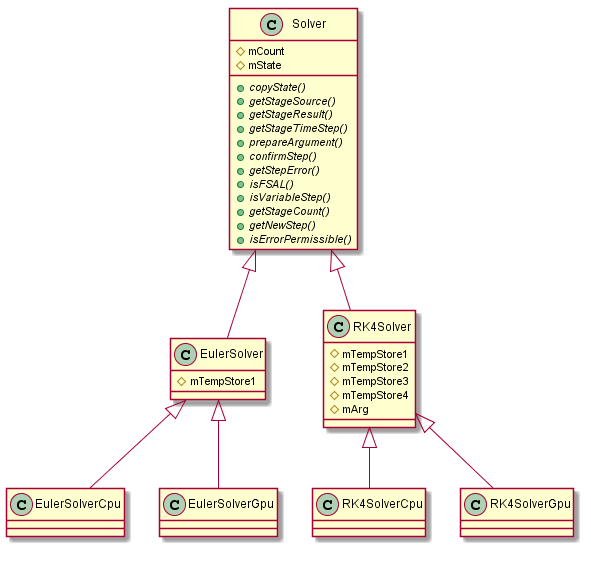
\includegraphics[width=0.8\linewidth]{solvers.png}}
	\caption{Иерархия наследования для методов численного решения.}
	\label{ris:solvers}
\end{figure}

\par EulerSolver, RK4Solver, DP45Solver являются потомками класса Solver и описывают основную информацию о реализуемых методах. Например, является ли данный численный метод методом с изменяемым шагом или требуется ли ему предварительная подготовка перед первой итерацией, сообщает количество итераций которые необходимы для данного метода (для метода Эйлера это значение равно единице). Кроме того, они хранят набор констант необходимых конкретно для данного метода, например для метода Рунге-Кутты это числа, используемые при вычислении нового состояния.
!!! информация о методе 
Все эти классы в полной мере реализуют все необходимые функции, описанные в классе предке, поэтому объект каждого из них можно создать. Именно они используются в качестве хранителей информации о выбранном методе решения задачи.

\par Классы EulerSolverCpu, EulerSolverGpu и другие уже являются потомками второго уровня, они наследуются от EulerSolver, RK4Solver, DP45Solver соответственно и предназначены для работы на центральном процессоре и видеокарте соответственно. Именно эти классы в полной мере реализуют выбранный численный метод.
\par Разберем работу данных классов на примере RK4SolverCpu. Фактически данный класс является большим хранилищем данных. Реализованный метод Рунге-Кутты предполагает четыре стадии, поэтому предок этого класса имеет четыре переменных для временного хранения данных (например mTempStore1, mTempStore2). Именно в них записывается информация о выделенных под хранилища ресурсах. В процессе работы от объекта данного класса можно получить источник и приемник информации в зависимости от стадии.
%Фактически подобные классы являются большими хранилищами для вычисляемых данных. Реализованный метод Рунге-Кутты предполагает четыре стадии выполнения, результат каждой стадии необходимо сохранять, а новое состояние вычисляется с использованием всех четырех результатов, полученных ранее. Данный класс при создании выделяет память под шесть матриц, которые будут использоваться при вычислениях, четыре временных хранилища, одна матрица, для текущего состояние и матрица, используемая при вычислении нового состояния. В процессе работы объект данного класса выдает в качестве источника или приемника информации либо временную матрица, либо матрицу состояния, в зависимости от текущей стадии выполнения. После завершения итерации вычисления выполняется пересчет нового состояния.

\newpage
\subsection{Класс Block и его потомки}

\par Класс Block и его потомки обеспечивают непосредственно расчеты, производимые с данными. Сам класс Block является абстрактным и, как следствие, его создание невозможно. Он описывает интерфейс для блоков, который позволит полноценно работать с реальными блоками - потомками данного класса. Кроме того, он имеет переменные для хранения всей необходимой информации о блоке, например, его положение в пространстве, размеры, тип и номер устройства, на котором блок будет выполняться. !!!(см. Рис.~\ref{ris:blocks}).

\begin{figure}[h]
	\center{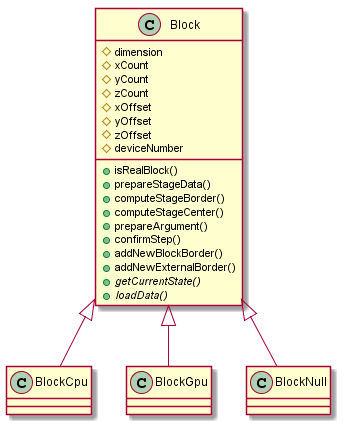
\includegraphics[width=0.6\linewidth]{blocks.png}}
	\caption{Иерархия наследования для блоков.}
	\label{ris:blocks}
\end{figure}

\par Класс BlockCpu является наследником класса Block, предназначенным для работы на центральном процессоре. Он является реальным блоком, который хранит информацию и осуществляет ее обработку. Для осуществления распараллеливания используется библиотека OpenMP.

\par Класс BlockGpu является наследником класса Block, предназначенным для работы на видеокарте. Он также является реальным блоком, но в отличии от класса BlockCpu всю информацию он хранит в памяти видеокарты, расчеты выполняются также на ней, для этого используется специальный язык CUDA.

\par Класс BlockNull единственный класс-наследник Block, который не является реальным блоком. Он нужен для того чтобы обозначить, что часть области, относящаяся к данному блоку на самом деле обрабатывается другим потоком и на другой машине. Но он позволяет выполнить все функции присущие блоку, но в данном случае ничего не будет выполнено. Кроме того, объект данного класса содержит основную информацию о блоке: его размеры и местоположение в пространстве.
%Основными классами приложения, которые занимаются непосредственно вычислениями на устройствах, являются потомки класса Block - BlockCpu и BlockGpu. Как можно догадаться из названия данных классов они предназначены для выполнения вычислений на центральном процессоре и видеокарте соответственно. Кроме того, присутствует класс BlockNull, который не выполняет вычислительной функции, а лишь хранит общую информацию о блоке, необходимую для 
корректной работы.

\newpage
\subsection{Класс Domain}

\par Главным управляющим классом приложения является класс Domain. Объект этого класса создается в единственном экземпляре каждым из потоков выполнения. Данный класс обладает широким набором возможностей. Чтение загрузочной информации из файла, во время которой фактически происходит инициализация всех переменных приложения. Вывод результатов вычисления как по завершению работы, так и во время выполнения. Также этот класс осуществляет сохранение текущего состояния вычислений и загрузку любого ранее сохраненного состояния, относящегося к той же задаче. !!!(см. Рис.~\ref{ris:all}).

\begin{figure}[h]
	\center{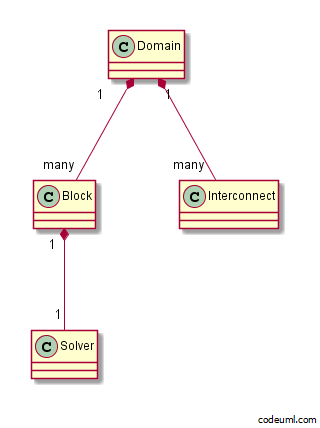
\includegraphics[width=0.6\linewidth]{all.png}}
	\caption{Общая архитектура приложения.}
	\label{ris:all}
\end{figure}

%\par Классами, которые определяют численные методы решения задачи, являются потомки класса Solver, например EulerSolver, RK4Solver или DP45Solver, эти классы хранят минимальный набор информации о методе Эйлера, методе Рунге-Кутты четвертого порядка и семистадийном методе Дормана-Принца. Их потомки, например EulerSolverCpu и EulerSolverGpu, создаются на центральном процессоре и видеокарте соотвественно и являются полноценной реализацей методов для работы на представленных устройствах.

\newpage
\subsection{Класс Interconnect}

\par Для пересылки данных между блоками, который расположены на разных узлах вычислительного кластера используется класс Interconnect. Каждый его экземпляр хранит номер потока, являющегося источником передаваемой информации, номер потока, который данную информацию должен принять, а также длину массива, который необходимо переслать. Экземпляры этого класса создаются на каждую связь между блоками каждым потоком. При вызове функции передачи/приема объект выполнит либо отправку сообщения, либо прием в зависимости от номера потока, который вызвал данную функцию у себя, либо не будет выполнено ничего, если пересылка осуществляться не должна, например поток не имеет к ней вообще никакого отношения, не является ни источником, ни приемником, либо пересылка для данной связи не требуется - блоки принадлежат одному потоку и, как следствие, расположены на одной машине и могут получать данные напрямую.

%\par Стоит отметить, что среди всех потоков выполнения главным считает поток с номером 0. Именно он собирает со всех данные и выполняет их сохранение, он же отвечает за вывод конечного результата вычислений, кроме того, он также участвует в вычислениях наряду с другими потоками.

\newpage
\section{Компоненты программного комплекса}

\par Приложение состоит из нескольких частей. Каждая из них отвечает за определенную часть работы, либо подготовительной, либо относящейся непосредственно к самим вычислениям, либо реализующей взаимодействие с пользователем.

\par Пользовательский интерфейс позволяет создавать и модифицировать проекты. Кроме того, он дает возможность управлять текущими вычислениями, а именно запускать, прекращать, приостанавливать, а также выполнять сохранение текущего состояния и его загрузку.

\par Часть предварительной обработки выполняет подготовку исходных данных. В ней происходит обработка геометрии и свойств области, производится определение размерности, расположения и размера блоков, граничных условий. Здесь же выполняется распределение блоков по вычислительным устройствам, формируется библиотека пользовательских функций.

\par Параллельный фреймворк и алгоритмы обработки данных составляют основу приложения и занимаются непосредственно самими вычислениями. К алгоритмам обработки данных относятся метод Эйлера, явные схемы Рунге-Кутты, методы Дормана-принца. Стоит отметить, что присутствует возможность расширения списка доступных методов решения.

\newpage
\section{Параллельный фреймворк}

%\par Параллельный фреймворк занимается непосредственной реализацией распределенных вычислений. С его помощью выполняется взаимодействие всех вычислительных устройств во время работы приложения. Он же реализует пересылку данных между блоками. Подобные пересылки необходимы в случае, когда одному блоку нужна информация от другого для продолжения собственных вычислений. Кроме того, фреймворк занимается обработкой событий, которые генерирует пользовательский интерфейс, а именно начало вычислений с заданными параметрами, приостановка вычислений, их прекращении, сохранение и загрузка состояний.

%\newpage
\subsection{Мелкозернистый параллелизм}

\par Мелкозернистый параллелизм осуществляется непосредственно на вычислительных устройствах. В зависимости от типа устройства будет использована библиотека OpenMP, для работы на центральном процессоре, и CUDA, в случае работы на видеокарте. Увеличение производительности достигается путем параллельного вычисления частей блока.

\par OpenMP реализует параллельные вычисления с помощью многопоточности, в которой <<главный>> (master) поток создает набор подчиненных (slave) потоков и задача распределяется между ними. Предполагается, что потоки выполняются параллельно на машине с несколькими процессорами (количество процессоров не обязательно должно быть больше или равно количеству потоков). Количество создаваемых потоков может регулироваться как самой программой при помощи вызова библиотечных процедур, так и извне, при помощи переменных окружения.

\par Данная библиотека работает в системах с общей памятью, поэтому каждая нить имеет доступ ко всем данным блока. Например, при расчете двумерного случая прямоугольник <<разрезается>> на полосы, обработка которых осуществляется одновременно. Библиотека OpenMP самостоятельно определяет количество таких полос и их ширину.

\par В качестве аналога данной библиотеки можно было использовать стандартные потоки языка C++, но подобный подход значительно усложнил бы разработку и увеличил вероятность ошибки. OpenMP обладает всеми необходимыми инструментами для реализации многопоточности на центральном процессоре в рамках одной машине и достаточно проста в использовании.

%\par Конкретно в данным случае библиотека осуществляет распараллеливание расчетов нового состояния блока. Каждой нити исполнения дается на обработку часть матрицы. Нить выполняет расчет новых значений основываясь на текущих данных своей части, кроме того она имеет возможность получить данные, которые обрабатывают другие нити, если таковые потребуются для расчета своих значений. Так как работа ведется с общей памятью никакой подготовки для такого <<чтения>> не требуется.

\par Как уже сообщалось ранее, при осуществлении вычислений на видеокарте используется CUDA - (Compute Unified Device Architecture) программно-аппаратная архитектура параллельных вычислений, которая позволяет существенно увеличить вычислительную производительность благодаря использованию графических процессоров фирмы Nvidia.

\par CUDA SDK позволяет программистам реализовывать на специальном упрощённом диалекте языка программирования Си алгоритмы, выполнимые на графических процессорах Nvidia, и включать специальные функции в текст программы на Си. Архитектура CUDA даёт разработчику возможность по своему усмотрению организовывать доступ к набору инструкций графического ускорителя и управлять его памятью.

\par При обработке блока на видеокарте каждая ячейка блока обрабатывается отдельным потоком. Каждый такой поток имеет необходимый доступ к данным.

\par В качестве альтернативы CUDA можно рассмотреть OpenCL, данный фреймворк для работы с графическими процессорами также предоставляет необходимые инструменты. Но так как CUDA разработана компанией Nvidia специально для своих видеокарт и, как следствие, она демонстрирует лучшие показатели производительности именно на видеокартах данной торговой марки. На вычислительный кластеры ставят подобные видеокарты, поэтому в качестве инструмента работы с видеокартами была выбрана именно CUDA.

\newpage
\subsection{Крупнозернистый параллелизм}

\par Крупнозернистый параллелизм осуществляется путем разбиения области на блоки и распределения блоков по вычислительным устройствам еще на этапе подготовки, о чем было изложено ранее. Данный подход позволяет использовать все вычислительные мощности имеющиеся в наличии и равномерно распределять нагрузку на устройства. На одном устройстве может располагаться несколько блоков одновременно, в таком случае их вычисление будет осуществляться в порядке очереди. Немаловажным фактом является то, что в случае если количество блоков значительно (в несколько раз) превышает количество вычислительных устройств, то блоки, которые имеют общие границы разумно располагать на одном устройстве, либо в пределах одной машины, а блоки не имеющих таких границ - на разных, сохраняя равномерность распределения блоков по устройствам в целом. Такой подход позволяет увеличить скорость расчетов для небольших, по количеству используемых узлов, областей. Достигается это уменьшение времени, которое необходимо на пересылку данных между блоками между итерациями вычислений, так как если блоки расположены на одном вычислительном устройстве или одной машине, то пересылка не будет выполняться в принципе, потому что данные уже доступны блоку. Очевидно, что в общем случае невозможно распределить все блоки таким образом чтобы пересылок не было вообще, но такой подход позволяет минимизировать количество пересылаемой информации, что положительно сказывается на производительности.

\newpage
\subsection{Пересылки информации}

\par Пересылка данных между разными машинами (вычислительными узлами) осуществляется с помощью библиотеки MPI. Message Passing Interface (MPI, интерфейс передачи сообщений) - программный интерфейс (API) для передачи информации, который позволяет обмениваться сообщениями между процессами, выполняющими одну задачу. MPI является наиболее распространённым стандартом интерфейса обмена данными в параллельном программировании, существуют его реализации для большого числа компьютерных платформ. Используется при разработке программ для кластеров и суперкомпьютеров. Основным средством коммуникации между процессами в MPI является передача сообщений друг другу. В стандарте MPI описан интерфейс передачи сообщений, который должен поддерживаться как на платформе, так и в приложениях пользователя. В первую очередь MPI ориентирован на системы с распределенной памятью, то есть когда затраты на передачу данных велики.




%Для автоматизации моделирования конечно-разностных диффузионных систем необходимо решить несколько задач. Среди них разработка инструмента моделирования уравнений (в том числе и уравнений с запаздыванием), которые были бы распределены в одномерных, двумерхных и трехмерных областях. Каждая область может быть представлена неким набором блоков. Для одномерного случая этими блоками являются отрезки, в случае плоскости - прямоугольник и, если область является трехмерной - параллелепипеды. Каждый из блоков характеризуется своими координатами в пространстве, размерами и информацией о своих границах. Граница блока может быть составлена из нескольких частей !!! Дирихле Нейман граница с другим блоком. !!!РИСУНКИ Кроме того, нужна поддержка соверенного оборудования , а именно неоднородных систем с иерархической организацией памяти. Также требуется высокий уровень абстракции, такой как автоматическая генерация кода по пользовательским функциям. !!! пользовательский интерфейс.

\par 
\end{document}


















